\documentclass[]{beamer}
% ----- PACCHETTI -----------
% Required for inserting images
\usepackage{graphicx} 
% Per i layout multicolonna
\usepackage{multicol}
% Colori listing codice
\definecolor{codegreen}{rgb}{0,0.6,0}
\definecolor{codegray}{rgb}{0.5,0.5,0.5}
\definecolor{codepurple}{rgb}{0.58,0,0.82}
\definecolor{backcolour}{rgb}{0.95,0.95,0.92}
% Sempre per lo pseudocodice
\usepackage{algorithm}
% Per lo pseudocodice
\usepackage{algpseudocode}
% Per scrivere listings codice
\usepackage{listings}    
\lstdefinestyle{mystyle}{
    language=Java,
    backgroundcolor=\color{backcolour},   
    commentstyle=\color{codegreen},
    keywordstyle=\color{magenta},
    numberstyle=\tiny\color{codegray},
    stringstyle=\color{codepurple},
    basicstyle=\ttfamily\footnotesize,
    breakatwhitespace=false,         
    breaklines=true,                 
    captionpos=b,                    
    keepspaces=true,                 
    numbers=left,                    
    numbersep=5pt,                  
    showspaces=false,                
    showstringspaces=false,
    showtabs=false,                  
    tabsize=2
}
\lstset{style=mystyle}
\lstset{linewidth=5.2cm}
% Per le regole di inferenza
\usepackage{ebproof}

% Bibliografia
% \addbibresource{Bibliography.bib}

% ------- FINE PACCHETTI --------
% -------- TEMA --------------
\usetheme{Warsaw}
\usecolortheme{seahorse}
% Per nascondere la barra di navigazione
\setbeamertemplate{navigation symbols}{}
% Per nascondere le sezioni in alto nelle slide
\setbeamertemplate{headline}{}
\setbeamertemplate{frame numbering}[fraction]
% Per i margini
% \setbeamersize{text margin left=8pt,text margin right=8pt} 
% Nuovo font
\newcommand\Fontvi{\fontsize{10}{7.2}\selectfont}
% ------ FINE TEMA --------
% ------- TITOLO ----------
\title{Dafny}
\subtitle{Un linguaggio per la verifica funzionale}
\author{Lorenzo Quellerba}
\institute{Università degli Studi di Torino}
\date{May 2023}
% ------- FINE TITOLO ----------
\begin{document}
\maketitle
% Cambia il titolo, Scaletta fa cagare
\begin{frame}{Contenuti}
    \tableofcontents
\end{frame}
% Verifica funzionale
\section{Introduzione alla verifica funzionale}
\begin{frame}{Introduzione alla verifica funzionale}
    \begin{itemize}
        \item La verifica funzionale è una tecnica di analisi statica
        \item L'obiettivo è quello di stabilire con rigore logico la correttezza di un programma relativamente alla specifica del suo comportamento
        \item Tradizionalmente, il processo di verifica avviene attraverso dimostrazioni su carta o mediante l'uso di proof assistant (processo lungo e che richiede esperienza)
        \item In particolare ci si concentra sull'automatizzazione del processo
    \end{itemize}
\end{frame}

% Qua fai discorso sull'automazione 
\begin{frame}[containsverbatim]{Introduzione alla verifica funzionale}\vspace{10pt}
Uno dei requisiti fondamentali alla base di una teoria per la verifica funzionale di programmi è la \textbf{modularità}
\begin{columns}[onlytextwidth]
    \column{0.5\pagewidth}
    \begin{center}
         \begin{lstlisting}
class C {
 var x:int;
 method i()
  ensures x>old(x)
 {x := x+1;}
}
        \end{lstlisting}
\end{center}
    \column{0.5\pagewidth}
    \begin{center}
        \begin{lstlisting}
class Client {
 method m0(c: C)
  ensures c.x>2*old(c.x)
 {
   c.x := 2*c.x;
   c.i();
 }
}
\end{lstlisting}
\end{center}
\end{columns}
\end{frame}

\begin{frame}[containsverbatim]{Introduzione alla verifica funzionale}
L'altro requisito è quello del supporto all'\textbf{incapsulamento}
\begin{columns}[onlytextwidth]
    \column{0.5\pagewidth}
    \begin{center}
         \begin{lstlisting}
class C {
 var x:int;
 method i()
  ensures getX() > old(getX())
 {x := x+1;}
 method getX()
 { return x;}
}
        \end{lstlisting}
\end{center}
    \column{0.5\pagewidth}
    \begin{center}
        \begin{lstlisting}
class Client {
 method m0(c: C)
  ensures c.getX()>2*old(c.getX())
 {
   c.x := 2*c.x;
   c.i();
 }
}
\end{lstlisting}
\end{center}
\end{columns}
\end{frame}
\subsection{Dafny, un linguaggio con supporto alla verifica funzionale}
\begin{frame}{Introduzione alla verifica funzionale}
    \begin{columns}[onlytextwidth]
        \column{0.5\textwidth}
         \begin{itemize}
        \item Si presenta Dafny, un linguaggio di programmazione imperativo orientato agli oggetti simile a Java
        \item Dafny supporta "nativamente" il processo di verifica attraverso \textit{keyword} dedicate all'interno del linguaggio alla definizione della specifica e un SMT solver che si occupa di dimostrare la validità delle verification conditions in modo (semi-)automatico
    \end{itemize}
        \column{0.5\textwidth}
        \begin{figure}[h]
            \centering
            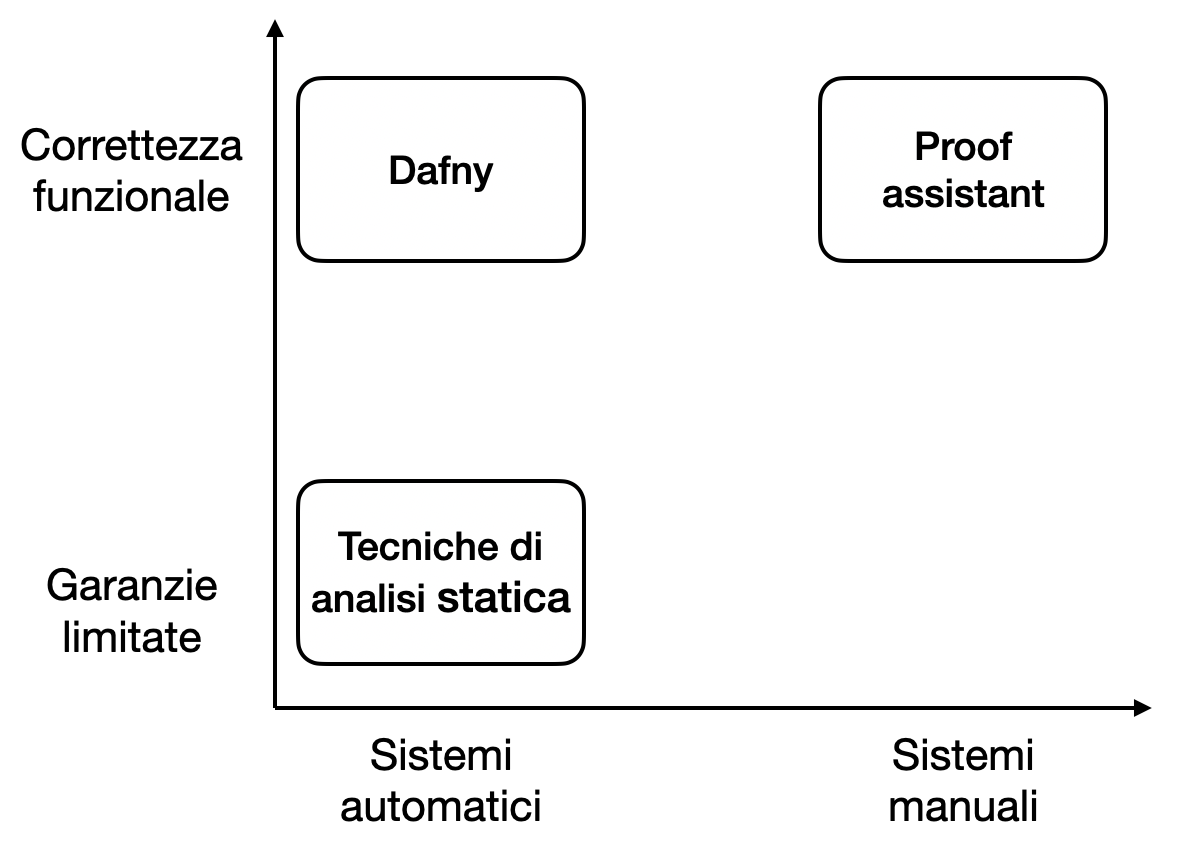
\includegraphics[scale=0.3]{assets/img/Levels_func_ver.png}
            \caption{Sistemi di analisi statica}
        \end{figure}
    \end{columns}
\end{frame}

\begin{frame}{Introduzione alla verifica funzionale}
L'architettura del sistema che si presenta è la seguente
\begin{figure}
    \centering
    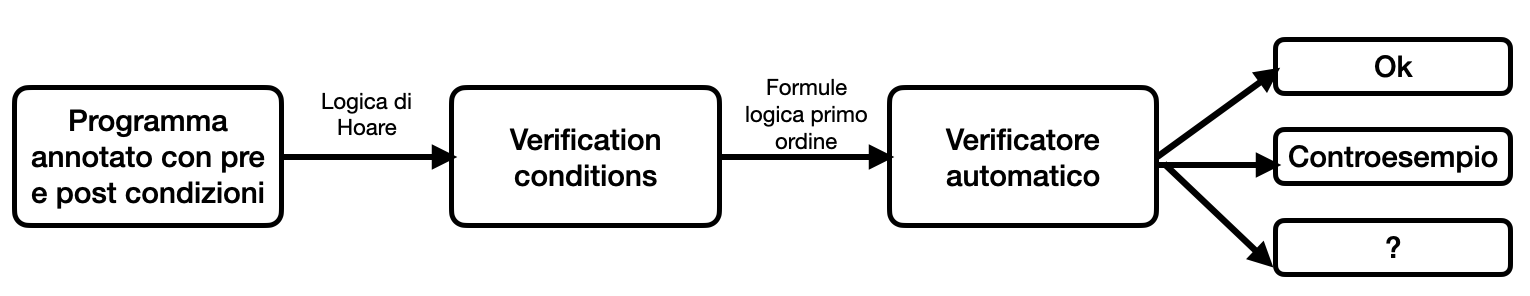
\includegraphics[scale=0.4]{assets/img/Processo_verifica.png}
    \caption{Processo di verifica}
    \label{fig:verification_process}
\end{figure}
\end{frame}


\section{Basi teoriche}
\subsection{Logica di Floyd-Hoare}
\begin{frame}[t]{Logica di Floyd-Hoare}
La logica di Floyd-Hoare è una logica di programma presentata come un sistema formale con assiomi e regole di inferenza\\
Il concetto alla base di tutto il sistema formale è quello della tripla di Hoare
\begin{center}
        \begin{block}{Tripla di Hoare}\vspace{4pt}
            \begin{center}
                \{P\} C \{Q\}
            \end{center}
            dove P è la precondizione, C è il programma e Q è la postcondizione
        \end{block}
\end{center}
A partire dalla tripla si definiscono le regole di inferenza e gli assiomi per tutti i costrutti
\begin{center}
        \begin{block}{Assegnamento}\vspace{4pt}
            \begin{center}
                \begin{prooftree}
                    \infer0[Asgn]{\{Q[E/x]\} x := E \{Q\}}
                \end{prooftree}
            \end{center}
        \end{block}
\end{center}
\end{frame}

\begin{frame}{Logica di Floyd-Hoare}
\begin{center}
        \begin{block}{Conseguenza}
            \begin{center}
                \begin{prooftree}
                    \hypo{P \rightarrow P'}
                    \hypo{$\{P'\} C \{Q'\}$}
                    \hypo{Q' \rightarrow Q}
                    \infer3[Conseq]{$\{P\} C \{Q\}$}
                \end{prooftree}
            \end{center}
        \end{block}
        \begin{block}{Composizione sequenziale}
            \begin{center}
                 \begin{prooftree}
                    \hypo{$\{P\}C1\{R\}$}
                    \hypo{$\{R\}C2\{Q\}$}
                    \infer2[Seq]{$\{P\} C1;C2 \{Q\}$}
                \end{prooftree}
            \end{center}
        \end{block}
        \begin{block}{Selezione}
            \begin{center}
                \begin{prooftree}
                    \hypo{\{P \land b\} C1 \{Q\}}
                    \hypo{\{P \land \neg b\} C2 \{Q\}}
                    \infer2[If]{\{P\} $IF b THEN C1 ELSE C2$ \{Q\}}
                \end{prooftree}
            \end{center}
        \end{block}
\end{center}
\end{frame}
\begin{frame}{Logica di Floyd-Hoare}
\begin{center}
    \begin{block}{Iterazione}
        \begin{center}
            \begin{prooftree}
                \hypo{\{P \land b\} C \{P\}}
                \infer1[While]{\{P\} $WHILE b DO C$ \{P \land \neg b\}}
            \end{prooftree}
        \end{center}
    \end{block}
\end{center}
\begin{example}
    Esempio di derivazione\\ \vspace{8pt}
    \scalebox{0.65}{
    \begin{prooftree}
            \hypo{x = 0 \rightarrow 2 + 1 = 3}
            \infer0[Asgn]{\{2 + 1 = 3\} y := 2 \{y + 1 = 3\}}
            \infer2[Asgn]{\{x = 0\} y := 2 \{y + 1 = 3\}}
            \infer0[Asgn]{\{y + 1\} x := y + 1 \{x = 3\}}
            \infer2[Conseq]{\{x = 0\} y := 2; x := y + 1 \{x = 3\}}
    \end{prooftree}
    }
\end{example}
\end{frame}

\begin{frame}{Logica di Floyd Hoare}
L'utilizzo della logica di Floyd-Hoare nella verifica funzionale risente di tre problemi
\begin{enumerate}
    \item l'assenza di una strategia esplicita per costruire una derivazione
    \item l'obbligo di dover dimostrare implicazioni logiche nella regola della conseguenza
    \item l'assenza di supporto alla \textit{modularità} del ragionamento se si introduce lo \textit{heap}
\end{enumerate}
\end{frame}

\subsection{Predicate transformer semantics}
\begin{frame}{Predicate transformer sematics}
\begin{itemize}
    \item La semantica dei \textit{predicate transformer} è un'idea introdotta da Dijkstra
    \item Definiscono la semantica di un linguaggio di programmazione assegnando ad ogni comando del linguaggio una funzione totale tra due predicati sullo spazio degli stati dei comandi
    \item Sono una riformulazione della logica di Hoare in delle strategie complete per costruire derivazioni valide
    \item Forniscono un algoritmo per ridurre il problema di verificare una tripla di Hoare nella verifica di una formula in logica del primo ordine
    \item Intuitivamente, fanno un esecuzione simbolica dei comandi trasformandoli in predicati
    \item Ne esistono due tipi \begin{itemize}
        \item la weakest precondition \textit{wp}
        \item la strongest postocondition \textit{sp}
    \end{itemize}
\end{itemize}
\end{frame}

\begin{frame}[t]{Predicate transformer semantics}
\begin{center}
    \begin{block}{Definizione \textit{wp}}
        Dato un comando \textit{C} e una postcondizione \textit{Q}, un predicato è la \textit{weakest precondition} se
        \begin{itemize}
            \item la tripla [wp(C,Q)]C[Q] è valida
            \item per ogni P tale per cui [P]C[Q] è valida allora P$\implies$wp(C,Q)
        \end{itemize}
    \end{block}
\end{center}
Si definisce una regola per il calcolo di \textit{wp} per ogni costrutto del linguaggio
\begin{center}
    \begin{block}{\textit{wlp} per l'assegnamento}
        \textit{wlp}(x:=e, Q) = Q[x/e]
    \end{block}
% Qua le definizioni dei singoli costrutti
    \begin{block}{\textit{wlp} per la composizione sequenziale}
        \textit{wlp}(C1;C2, Q) = \textit{wlp}(C1, \textit{wlp}(C2,Q))
    \end{block}
\end{center}
\end{frame}

\begin{frame}[t]{Predicate transformer semantics}
\begin{center}    
    \begin{block}{\textit{wlp} per la selezione}
        \textit{wlp}(IF b THEN C1 ELSE C2, Q) = (b$\implies$\textit{wlp}(C1,Q)) $\land$ ($\neg$b$\implies$\textit{wlp}(C2,Q))
    \end{block}
    \begin{block}{\textit{wlp} per l'iterazione}
        \textit{wlp}(WHILE \{I\} b DO C, Q) = I, dove I rappresenta l'invariante
    \end{block}
\end{center}
Per verificare che $\models$\{P\}C\{Q\} quindi
\begin{enumerate}
    \item si calcola \textit{wp}(C,Q)
    \item si verifica che l'implicazione P$\implies$\textit{wp}(C,Q) sia \textbf{valida}
\end{enumerate}
\end{frame}
\subsection{Frame problem}
\begin{frame}{Frame problem}
\begin{block}{Frame problem}
    \textit{Descrivendo formalmente i cambiamenti in un sistema, come specificare quali parti dello stato del sistema non sono influenzate dal cambiamento?}
\end{block}
\begin{itemize}
    \item In un contesto modulare è un problema particolarmente complesso
\end{itemize}
\end{frame}

\begin{frame}[containsverbatim]{Frame problem}
\lstset{linewidth=11cm}
\begin{lstlisting}
class Node {
  var v:int;
  var next:Node;
}
class List {
  var c: Node;
  
  constructor()
    ensures len() == 0
  {c := null;}
  
  function len() returns int 
  {len_aux();}
  
  function len_aux(p:Node) returns int
  {
    p = null ? 0 : 1+len_aux(p.next)
  }
}\end{lstlisting}
\end{frame}

\begin{frame}[containsverbatim]{Frame problem}
\lstset{linewidth=11cm}
\begin{lstlisting}
var A,B : List;
A := new List;
B := new List;
assert A.len() == 0;
\end{lstlisting}
\begin{itemize}
    \item Dimostrare che l'asserzione è vera è impossibile
    \item Il costruttore assicura che \textit{len() == 0} ma non garantisce nulla rispetto a ciò che potrebbe succedere durante \textit{B := new List;} (ad esempio modifiche a \textit{A.c})
    \item Non c'è un modo per esprimere che "nessuna variabile del client è interessata dalla modifica" perché le variabili del client sono sconosciute
    \item Non è possibile esprimere il fatto che solo il campo \textit{c} del nuovo oggetto è modificato, il client non conosce i dettagli implementativi interni
    \item Non c'è un modo per esprimere la presenza o l'assenza di \textit{abstract aliasing}
\end{itemize}
\end{frame}
\subsection{Dynamic Frames}
\begin{frame}{Dynamic Frames \cite{Dfav}}
\begin{itemize}
    \item L'idea alla base dei dynamic frames è quella dell'introduzione dei \textit{footprint} di metodi e funzioni
    \item Il \textit{footprint} rappresenta l'insieme di campi che un un metodo o una funzione può leggere o modificare (intuitivamente, l'insieme di locazioni di memoria da cui dipende nel calcolo)
    \item Nel caso di un metodo si introduce la keyword \textit{modifies}, nel caso di una funzione la keyword \textit{reads}
\end{itemize}
\begin{block}{Dynamic frames}
    Un \textit{dynamic frame} è una funzione pura la cui valutazione produce un insieme di campi (una \textit{\textbf{regione}})
\end{block}
\end{frame}

\begin{frame}{Dynamic Frames}
    \begin{itemize}
        \item Con l'aggiunta del \textit{footprint} è ora possibile verificare l'asserzione mostrata in precedenza, è sufficiente garantire che il \textit{footprint} del metodo \textit{len()} è disgiunto da quello del costruttore di \textit{B}
        \item Allo stesso modo è ora possibile per esempio esprimere proprietà come l'assenza di cicli all'interno della lista, proprietà che prima erano inesprimibili
        \item L'aggiunta dei \textit{footprint} però non è sufficiente, sono necessarie altre due convenzioni \begin{itemize}
            \item \textit{swinging pivots}
            \item \textit{self framing}
        \end{itemize}
    \end{itemize}
\end{frame}

\begin{frame}[containsverbatim]{Swinging pivots}
\begin{block}{Swinging pivots}
    Sia \textit{S} l'insieme di dynamic frames presenti nel \textit{footprint} di un metodo. Il valore di qualsiasi dynamic frame in \textit{S} può essere aumentato solo da locazioni presenti in qualche altro dynamic frame in \textit{S} o da posizioni appena allocate
\end{block}
\lstset{linewidth=11cm}
\begin{lstlisting}
// Nel footprint e' presente solo repr(): il suo valore 
// puo' essere incrementato solo da nuove locazioni
method insert(x:int)
    modifies repr()
// Nel footprint sono presenti repr() e p.repr(). 
// repr() puo' essere aumentato solo da locazioni 
// precedentemente in p.repr() o da nuove locazioni
method prepend(p:List)
    reads p.repr()
    modifies repr()
\end{lstlisting}
Per esprimere questa convenzione si fa ricorso alla keyword \textit{\textbf{fresh}}
\end{frame}

\begin{frame}[containsverbatim]{Self framing}
\begin{block}{Self framing}
    Dynamic frames che sono sconosciuti ad un metodo \textit{m} e che sono disgiunti dal suo footprint, non devono cambiare quando \textit{m} è invocato: il footprint di un dynamic frame deve essere il dynamic frame stesso
\end{block}    
\lstset{linewidth=11cm}
\begin{lstlisting}
function rep() returns reg
    reads rep();
{ rep_aux(); }

function rep_aux(p: Node) returns reg
    reads rep_aux()
{ p = null? {} : {p.v, p.n} + rep_aux(p.n); }
\end{lstlisting}
\end{frame}

\section{Dafny}
\subsection{Introduzione a Dafny}
\begin{frame}{Introduzione a Dafny}
\begin{columns}[onlytextwidth]
\column{0.75\textwidth}
\begin{itemize}
    \item Il linguaggio è stato ideato da Rustan Leino durante il suo lavoro presso Microsoft Research
    \item Supporta sia il paradigma imperativo che quello funzionale
    \item La specifica formale viene formulata al suo interno attraverso pre-post condizioni, invarianti di ciclo, metriche per la terminazione e una implementazione dei dynamic frames (il nome Dafny nasce dalla permutazione di alcune lettere di \textit{dynamic frames})
    \item Il supporto per l'interazione con l'utente è quasi inesistente fatto salve per l'istruzione \textit{print}
\end{itemize}
\column{0.25\textwidth}
\begin{figure}
    \centering
    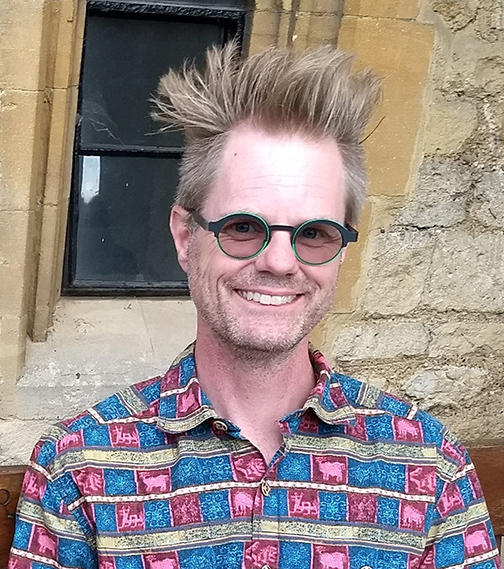
\includegraphics[scale=0.2]{assets/img/Rustan-feature.jpg}
    \caption{Rustan Leino}
    \label{fig:my_label}
\end{figure}
\end{columns}
\end{frame}

\subsection{Architettura}
\begin{frame}{Architettura del sistema}
\begin{itemize}
    \item In questa presentazione si fa riferimento alla versione 3.12 del linguaggio
    \item I file Dafny hanno estensione .\textit{dfy}
    \item L'installazione di Dafny in realtà non installa solo il linguaggio col suo compilatore ma l'intero sistema sottostante dedicato alla verifica
\end{itemize}
\begin{figure}
    \centering
    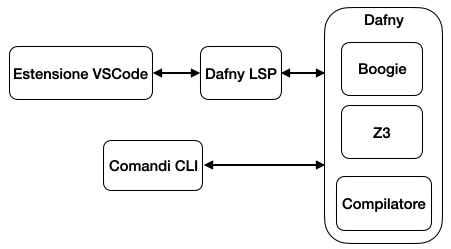
\includegraphics[scale=0.5]{assets/img/Dafny_schema.png}
    \caption{Componenti del sistema Dafny}
\end{figure}
\end{frame}

\begin{frame}{Architettura del sistema}
\begin{figure}
    \centering
    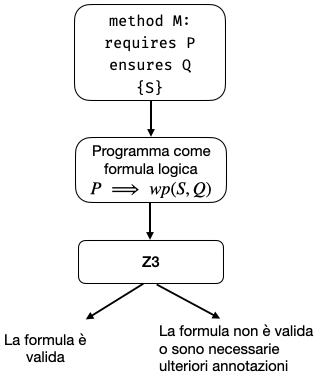
\includegraphics[scale=0.5]{assets/img/verification_schema.png}
    \caption{Processo di verifica}
\end{figure}
\end{frame}

\subsection{Boogie}
\begin{frame}{Boogie}
\begin{itemize}
    \item Boogie è un linguaggio intermedio di verifica creato da Microsoft Research
    \item È progettato per essere un layer intermedio per la costruzione di verificatori di programmi per altri linguaggi (VCC, Dafny, Chalice)
    \item Ci sono sostanzialmente due motivi per utilizzare un linguaggio intermedio\begin{itemize}
        \item lo sviluppo del linguaggio "front-end" è indipendente dalla metodologia di verifica
        \item non è necessario che il verificatore sia in grado di comprendere la semantica di linguaggi diversi, è sufficiente che comprenda Boogie
    \end{itemize}
\end{itemize}
\end{frame}

\begin{frame}[containsverbatim]{Boogie}
    \begin{itemize}
        \item La sintassi e le caratteristiche di Boogie sono altamente tecniche, per comprenderne ad alto livello il funzionamento si riporta un esempio \cite{SMT_applications}
    \end{itemize}
\lstset{linewidth=11cm}    
\begin{lstlisting}[basicstyle=\tiny]
int BinarySearch(int[] a, int len, int key)
// precondizione: 0 <= len <= |a| and forall i :: 0 <= i <= len - 2 and
// forall j :: i + 1 <= j <= len - 1 ==> a[i] < a[j]
{
    int low = 0;
    int high = len;
    while (low < high)
    // invariante: 0 <= low <= high <= len <= |a| and
    // forall i :: 0 <= i <= low - 1 ==> a[i] < key and
    // forall i :: high <= i <= len - 1 ==> a[i] > key
    { 
        //Ricerca dell'elemento mediano
        int mid = low + (high - low) / 2;
        int val = a[mid];
        if (key < val) {
            low = mid + 1;
        } else if (val < key) {
            high = mid;
        } else {
            return mid;
        }
    }
    return -1;
}
// postcondizione: (0 <= result ==> a[result] = key) and 
// (result < 0 ==> forall i :: 0 <= i <= len - 1 ==> a[i] != key)
\end{lstlisting}
\end{frame}

\begin{frame}[containsverbatim]{Boogie}
\begin{itemize}
    \item La semantica di ogni costrutto del linguaggio "ad alto livello" è definita in termini del linguaggio intermedio
    \item Ad esempio,
\end{itemize}
\lstset{linewidth=11cm}   
\begin{lstlisting}
// if (cond) S; else T;
{assume cond; S;} [] {assume !cond; T;}
// while (cond) inv S[x,y] dove x e y sono le variabili di programma modificate dal loop
assert inv; // controllo invariante in entrata
havoc x,y;  // salto ad una interazione arbitraria
assume inv;
{
    assume guard;
    S;
    assert inv; // controllo che l'invariante sia mantenuta
    assume false;
    []
    assume !guard; //uscita dal loop
}
\end{lstlisting}
\end{frame}

\begin{frame}[containsverbatim]{Boogie}
\lstset{linewidth=11cm}   
\begin{lstlisting}[basicstyle=\tiny]
int BinarySearch(int[] arr, int len, int key){
    l1: assume pre
    l2: int low = 0;
    l3: int high = len;
    l4: assert inv;
    l5: havoc low, high;
    l6: assume inv;
    l7: {
        m1: assume (low < high);
        // Ricerca dell'elemento mediano
        int mid = low + (high - low) / 2;
        int val = a[mid];
        m2: {
            n1: assume (key < val);
            n2: low = mid + 1;
            []
            n3: assume !(key < val);
            n4: assume (val < key);
            n5: high = mid;
            []
            n6: assume !(key < val);
            n7: assume !(val < key);
            n8: assert post[result := mid]
            n9: assume false
        }
        m3: assert inv:
        m4: assume false;
        []
        m5: assume !(low < high);
    }
    l8: assert post[result := -1]
}
\end{lstlisting}
\end{frame}

\begin{frame}{Boogie}
\begin{figure}
    \centering
    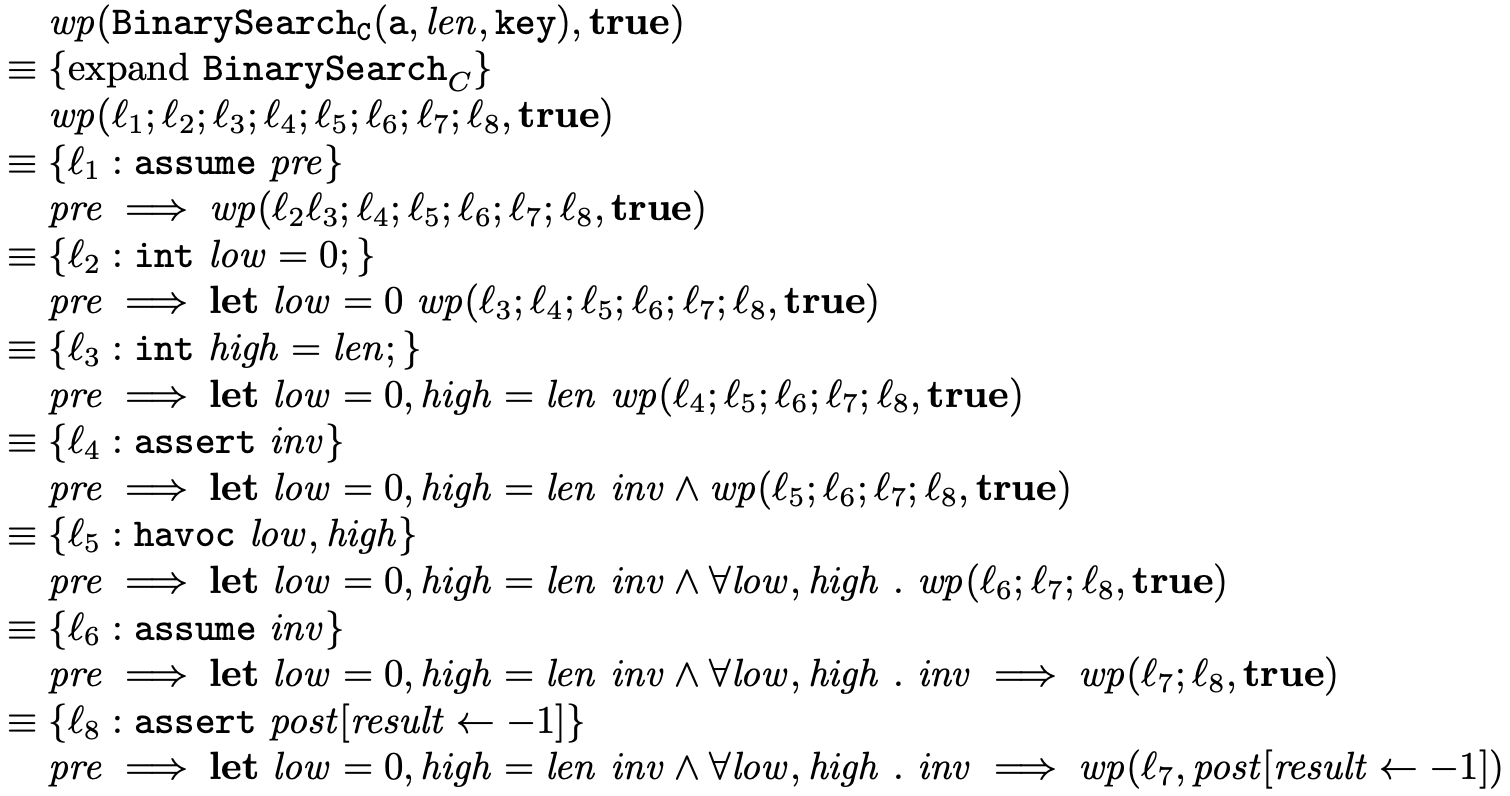
\includegraphics[scale=0.4]{assets/img/wp1.png}
\end{figure}
\end{frame}

\begin{frame}{Boogie}
\begin{figure}
    \centering
    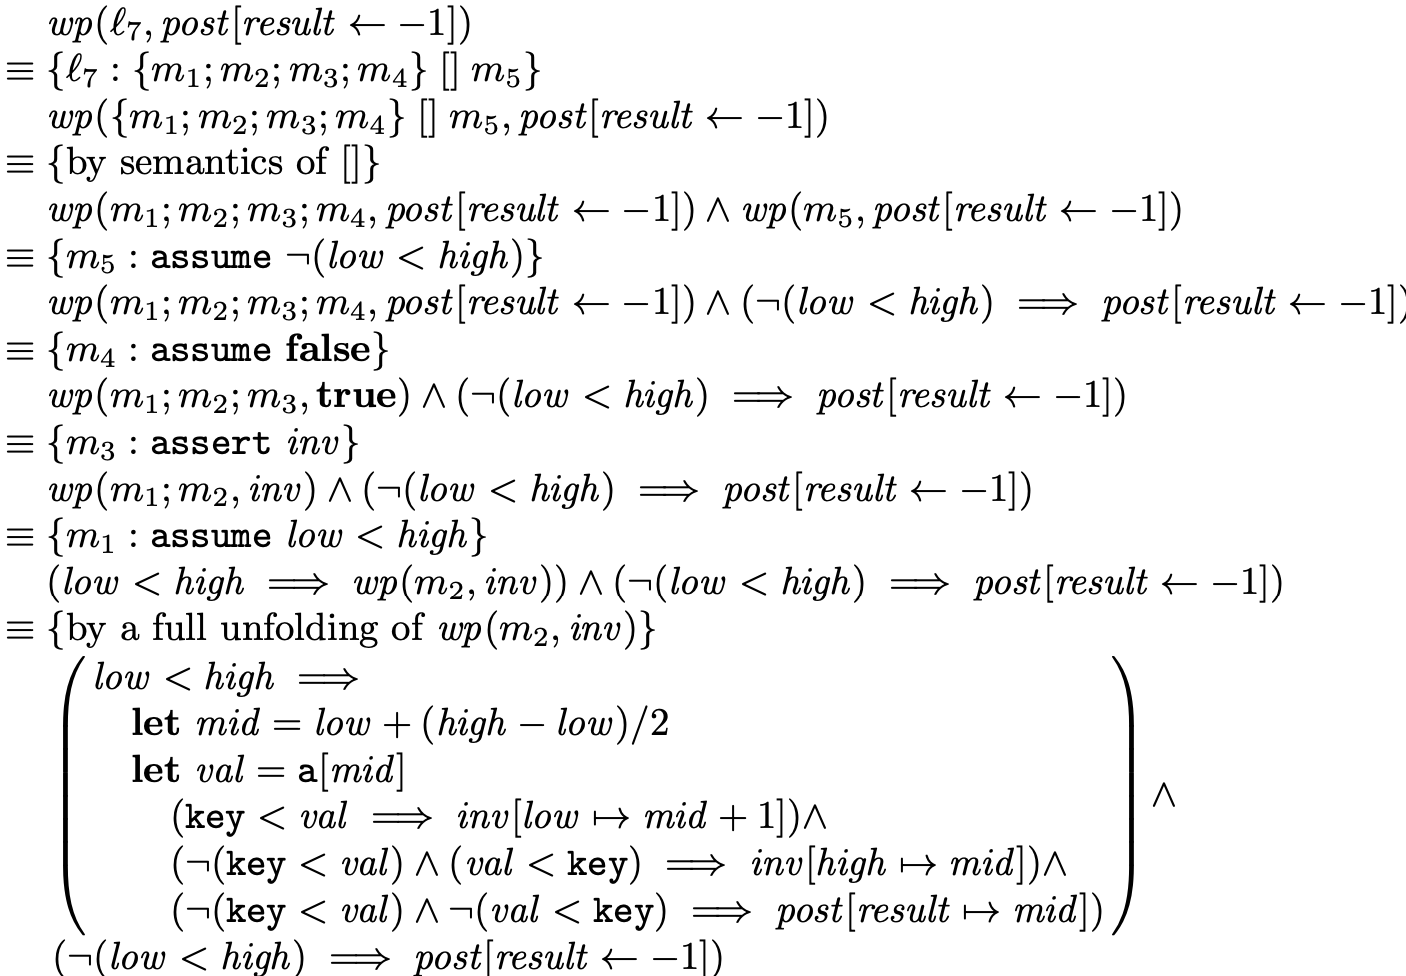
\includegraphics[scale=0.4]{assets/img/wp2.png}
\end{figure}
\end{frame}

\begin{frame}{Boogie}
\begin{figure}
    \centering
    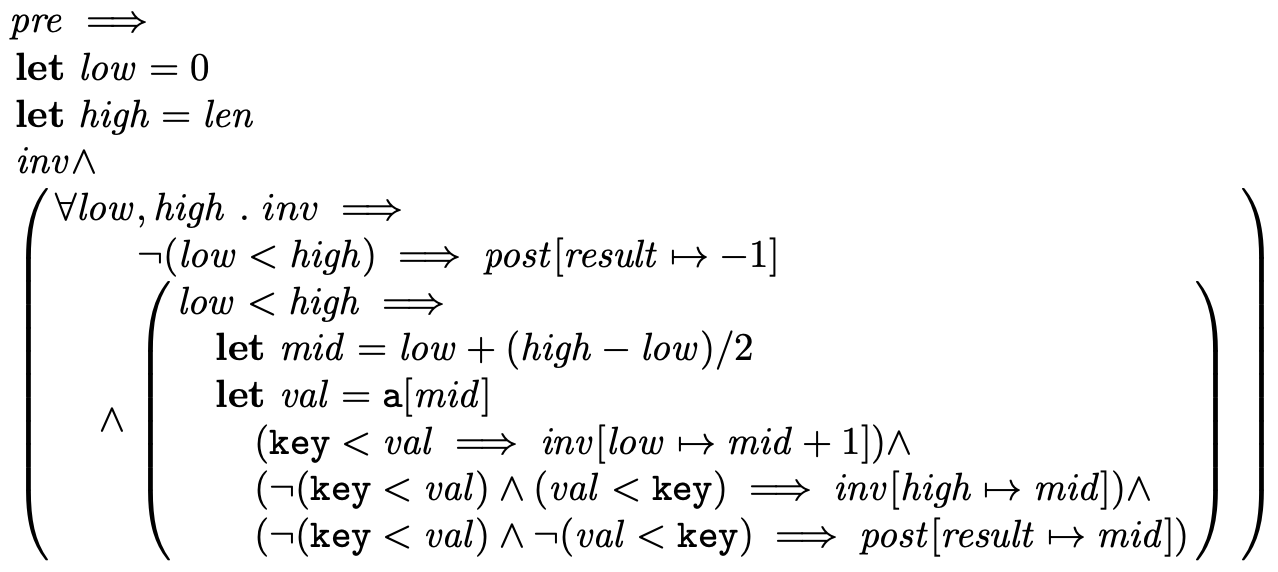
\includegraphics[scale=0.5]{assets/img/wp3.png}
\end{figure}
\begin{itemize}
    \item Questa formula rappresenta il programma sottoforma di formula logica che deve essere risolta dall'SMT solver
\end{itemize}
\end{frame}

\subsection{Z3}
\begin{frame}{Z3}
\begin{columns}[onlytextwidth]
\column{0.7\textwidth}
\begin{itemize}
    \item Z3 è un SMT solver progettato dal gruppo RiSE (Research in Software Engineering) di Microsoft Research
    \item È stato sviluppato per risolvere problemi della verifica di programmi
    \item Tra le teorie supportate sono presenti \begin{itemize}
        \item aritmetica lineare
        \item array, liste
        \item funzioni non interpretate
        \item uguaglianze
        \item quantificatori
    \end{itemize}
\end{itemize}
\column{0.3\textwidth}
\begin{figure}
    \centering
    
\includegraphics[scale=0.25]{assets/img/z3.jpg}
\end{figure}
\end{columns}
\end{frame}

\begin{frame}{SMT solver per la verifica funzionale}
\begin{itemize}
    \item L'obiettivo è stabilire la validità di una formula \textit{$\phi$}
    \item Il problema della dimostrazione di validità di una formula si può ridurre al problema di dimostrare l'insoddisfaciblità  di $\neg$\textit{$\phi$}
    \item Un SMT solver estende il problema della soddisfacibilità di una formula in logica proposizione (SAT problem) ad una formula \textit{FOL} attraverso le \textit{teorie}
\end{itemize}
\begin{figure}
    \centering
    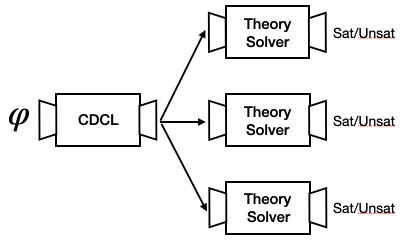
\includegraphics[scale=0.5]{assets/img/theory_solver.png}
\end{figure}
\end{frame}

\begin{frame}{SMT solver per la verifica funzionale}
\begin{itemize}
    \item Intuitivamente il funzionamento può essere schematizzato nel seguente modo
\end{itemize}
\begin{figure}
    \centering
    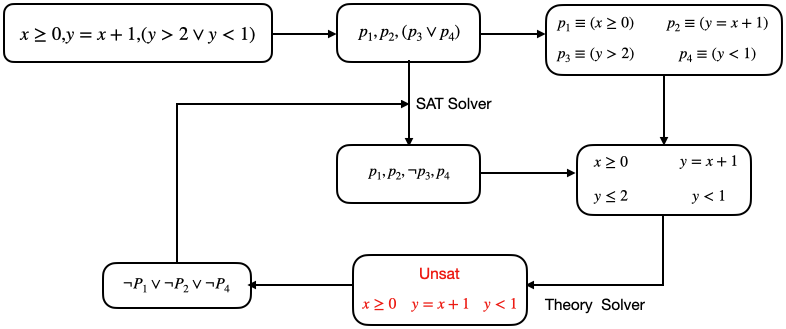
\includegraphics[scale=0.4]{assets/img/smt.png}
\end{figure}    
\end{frame}

\begin{frame}{Un semplice esempio \cite{SMTsolver_ex}}
\begin{example}
\begin{enumerate}
    \item[1] Si supponga di partire dalla congiunzione delle seguenti formule:\\
    $f(f(x)-f(y)) = a$\\
    $f(0)=a+2$\\
    $x = y$\\
    \item[2] La formula contiene sia aritmetica lineare che la teoria delle funzioni non interpretate, vanno separate attraverso la \textit{purificazione}\\
    $f(e_1)=a$\\
    $e_1 = f(x)-f(y)$
    \item[3] A sua volta $e_1$ può ulteriormente essere scomposta in\\
    $e_1 = e_2-e_3$\\
    $e_2 = f(x)$\\
    $e_3 = f(y)$
\end{enumerate}
\end{example}
\end{frame}

\begin{frame}{Un semplice esempio}
\begin{example}
    \begin{enumerate}
    \item[4] Lo stesso procedimento si applica per $f(0)=a+2$\\
    $f(e_4)=e_5$\\
    $e_4=0$\\
    $e_5=a+2$
    \item[5] Ora le formule sono scomposte in due teorie:\begin{itemize}
        \item Quelle nella teoria delle funzioni non interpretate\\
        $f(e_1)=a$\\
        $e_2=f(x)$\\
        $e_3=f(y)$\\
        $f(e_4)=e_5$\\
        $x=y$\\
        \item Quelle nella teoria dell'aritmetica\\
        $e_1=e_2-e_3$\\
        $e_4=0$\\
        $e_5=a+2$\\
        $x=y$
    \end{itemize} 
    \end{enumerate}
\end{example}
\end{frame}

\begin{frame}{Un semplice esempio}
\begin{example}
    \begin{enumerate}
        \item[6] Considerando le formule nella teoria delle funzioni non interpretate, nella teoria è contenuta una regola che afferma che se $x=y$ allora $f(x)=f(y)$. Applicando la regola si ottiene  $f(x)=f(y)$ e siccome $f(x)=e_2$ e $f(y)=e_3$ allora $e_2=e_3$
        \item[7] L'uguaglianza $e_2=e_3$ viene aggiunta all'insieme di formule della teoria dell'aritmetica
        \item[8] A questo punto il risolutore della teoria dell'aritmetica può scoprire che $e_2-e_3=0$ e che quindi $e_1=e_4$
        \item[9] Questa scoperta viene restituita al risolutore della teoria delle funzioni non interpretate da cui si ottiene che $a=e_5$
    \end{enumerate}
\end{example}
\end{frame}

\begin{frame}{Un semplice esempio}
\begin{example}
 \begin{enumerate}
        \item[10] L'insieme finale di vincoli è il seguente (interamente nella teoria dell'aritmetica)\begin{itemize}
            \item $e_1=e_2-e_3$
            \item $e_4=0$
            \item $e_5=a+2$
            \item $x=y$
            \item $e_2=e_3$
            \item $a=e_5$
        \end{itemize}
        \item[11] $a=e_5$ e al tempo stesso $e_5=a+2$, da cui si conclude che la formula originaria è insoddisfacibile
    \end{enumerate}
\end{example}
\end{frame}

\begin{frame}{SMT solver per la verifica funzionale}
    \begin{figure}
        \centering
        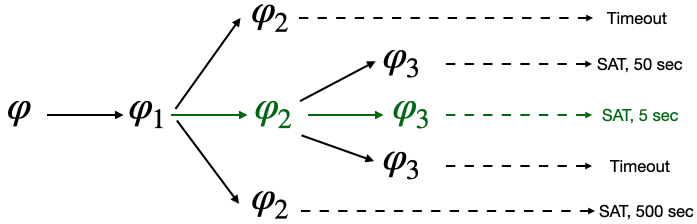
\includegraphics[scale=0.45]{assets/img/search_space.png}
    \end{figure}
\end{frame}

\subsection{Approfondimento linguaggio Dafny}
\begin{frame}{Anatomia di un programma Dafny}
    Un programma Dafny è composto da 4 "blocchi" fondamentali \cite{Dafny_ref_manual}
    \begin{itemize}
        \item Funzioni
        \item Predicati
        \item Metodi
        \item Classi
    \end{itemize}
\end{frame}

\begin{frame}[containsverbatim]{Funzioni}
\lstset{linewidth=11cm}
\begin{lstlisting}
function Nome<T>(a: A, b: B): T
    requires _precondizione_
    reads _frame di memoria_
    ensures _postcondizione_
    decreases _metrica di terminazione_
{
    Corpo
}
\end{lstlisting}
\begin{itemize}
    \item Le funzioni sono \textit{ghost} di default a meno che non vengano definite come \textit{function method}
    \item Sono funzioni nel senso matematico, non possono avere \textit{side-effects}
\end{itemize}
\end{frame}

\begin{frame}[containsverbatim]{Predicati}
\lstset{linewidth=11cm}
\begin{lstlisting}
predicate sorted(a: array<int>)
    reads a
{
forall j, k :: 0 <= j < k < a.Length ==> a[j] <= a[k]
}
\end{lstlisting} 
\begin{itemize}
    \item Sono identici alle funzioni ma possono ritornare esclusivamente un valore booleano
\end{itemize}
\end{frame}

\begin{frame}[containsverbatim]{Metodi}
\lstset{linewidth=11cm}
\begin{lstlisting}
method Nome<T>(a: A, b: B) returns (x: X, y: Y)
    requires _precondizione_
    modifies _frame di memoria_
    ensures _postcondizione_
    decreases _metrica di terminazione_
{
    Corpo
}
\end{lstlisting}   
\begin{itemize}
    \item Vari tipi di metodi (costruttori, lemmi, lemmi \textit{twostate}..)
    \item Può essere reso \textit{ghost} attraverso la dichiarazione \textit{ghost method}
    \item Non è necessario \textit{return esplicito}, i parametri in input sono immutabili
\end{itemize}
\end{frame}

\begin{frame}[containsverbatim]{Classi}
\lstset{linewidth=11cm}
\begin{lstlisting}[basicstyle=\tiny]
class Nome
{
    var nome: tipo
    constructor(x: tipo)
        ensures _postcondizione_
    {
        Corpo
    }
    predicate Valid()
        reads _frame di memoria_
    {
        Corpo
    }
    method NomeMetodo(y: tipo)
        requires _precondizione_
        modifies _frame di memoria_
        ensures _postcondizione_
        decreases _metrica di terminazione_
    {
        Corpo
    }   
}
\end{lstlisting}
\begin{itemize}
    \item Identiche ad altri linguaggi di programmazione (ad esempio Java) fatta eccezione per il \textit{subclassing}
\end{itemize}
\end{frame}

\begin{frame}{Keyword per la specifica funzionale}
    \begin{itemize}
        \item Il supporto alla verifica funzionale è reso possibile dalle \textit{keyword} riservate alla specifica del comportamento: \begin{itemize}
            \item \textit{requires}
            \item \textit{ensures}
            \item \textit{decreases}
            \item \textit{invariant}
            \item \textit{assert}
            \item \textit{assume}
            \item \textit{reads}
            \item \textit{modifies}
        \end{itemize}
    \end{itemize}
\end{frame}

\begin{frame}[containsverbatim]{\textit{requires}}
    \begin{itemize}
        \item Rappresenta la precondizione
        \item Se viene omessa, si assume \textit{true}
        \item Se la precondizione è particolarmente lunga è possibile dividerla in più \textit{requires} diverse che vengono considerate come se fossero in congiunzione tra di loro
        \item Il verificatore controlla che la precondizione sia soddisfatta ad ogni chiamata
    \end{itemize}
\lstset{linewidth=11cm}
\begin{lstlisting}
method FindMax(a: array<int>) returns (i:int)
    requires a.Length >= 1
\end{lstlisting}
\end{frame}

\begin{frame}[containsverbatim]{\textit{ensures}}
\begin{itemize}
    \item Simmetrica a \textit{requires}, rappresenta la postcondizione
\end{itemize}    
\lstset{linewidth=11cm}
\begin{lstlisting}
method Find(a:array<int>, key:int) returns (index:int)
    ensures 0 <= nidex ==> index < a.Length && 
    a[index] == key
    ensures index < 0 ==> forall k :: 
    0 <= k < a.Length ==> a[k] != key
\end{lstlisting}
\end{frame}

\begin{frame}[containsverbatim]{\textit{decreases} }
    \begin{itemize}
        \item La keyword \textit{decreases} è dedicata alla terminazione
        \item L'idea è quella di annotare ogni iterazione di un ciclo (o ogni chiamata ricorsiva) con un valore per cui esista una relazione d'ordine (ossia per cui non esistono catene discendenti infinite) e assicurarsi che iterazioni successive decrementino l'etichetta
        \item L'etichetta prende il nome di \textit{variant}
        \item Si faccia riferimento al seguente esempio di una funzione che calcola la somma di una lista di numeri interi \cite{Decreases_ex}
    \end{itemize}
    \lstset{linewidth=11cm}
\begin{lstlisting}
function Sum(xs: seq<int>): int
    decreases xs;
{
    if xs == [] then 0 else xs[0] + Sum(xs[1..])
}
\end{lstlisting}
\end{frame}

\begin{frame}{\textit{invariant}}
    \begin{itemize}
        \item Rappresenta il concetto di invariante per un ciclo
        \item Esattamente come da definizione, deve essere un'asserzione valida rispettivamente \begin{itemize}
            \item subito prima dell'ingresso nel ciclo
            \item alla fine dell'esecuzione del corpo del ciclo
            \item all'uscita dal ciclo
        \end{itemize}
    \end{itemize}
\end{frame}

\begin{frame}{\textit{assert}}
\begin{itemize}
    \item Utilizzata principalmente in fase di \textit{debug} per sincerarsi che certe proprietà che sono "evidenti" per l'utente siano dimostrabili anche dal verificatore
    \item Sono \textit{ghost statements}
    \item Talvolta sono necessarie per guidare il processo di verifica
\end{itemize}    
\end{frame}

\begin{frame}{\textit{assume}}
    \begin{itemize}
        \item Utilizzata durante la costruzione di una prova
        \item Permette la specifica di una formula che il verificatore assumerà come vera senza la necessità di una prova
        \item Utile per rimandare la verifica di sottoproblemi nell'ambito di una prova più grande
        \item Un programma contente \textit{assume} non può essere compilato
    \end{itemize}
\end{frame}

\begin{frame}{Un semplice esempio: successione di Fibonacci}
    \begin{itemize}
        \item Come primo semplice programma consideriamo l'implementazione di un metodo che calcoli l'\textit{n}-esimo numero della successione di Fibonacci
        \item La definizione matematica è $F_n = F_{n-1} + F_{n-2}$ con $F_1 = F_2 = 1$ e $F_0 = 0$. 
        \item Implementarla direttamente in questo modo avrebbe complessità esponenziale
        \item L'idea è quella di utilizzare un contatore e calcolare ripetutamente coppie adiacenti di numeri della sequenza fino a quando non viene raggiunto il numero desiderato
    \end{itemize}
\end{frame}

\subsection{Ricerca binaria}
\begin{frame}{Un semplice esempio: BinarySearch}
    \begin{itemize}
        \item L'algoritmo di ricerca binaria trova l'indice in cui è presente una chiave all'interno di un array ordinato in tempo logaritmico nel caso peggiore
    \end{itemize}
\begin{algorithm}[H]
\caption{BinarySearch(A[0..n], key)}\label{alg:bin_search}
    \begin{algorithmic}\scriptsize
        \Require L'array $A$ è ordinato in ordine non decrescente
        \Ensure Se $key$ è contenuto in $A$ restituisce l'indice della sua posizione, -1 altrimenti
        \State $low \gets 0$
        \State $high \gets n$
        \While{$low < high$}\\
            \Comment{Invariant: Se la chiave è in A[0..n] allora la chiave è in A[low..high]}
            \State $mid \gets (low + high) / 2$
            \If{$key > A[mid]$}
                \State $low \gets mid + 1$
            \ElsIf{$key < a[mid]$}
                \State $high \gets mid$
            \Else
                \State \textbf{return} $mid$
            \EndIf
        \EndWhile
        \State \textbf{return} $-1$
    \end{algorithmic}
\end{algorithm}
\end{frame}

\subsection{Dynamic frames in Dafny}
\begin{frame}{Implementazione dei dynamic frames}
\begin{itemize}
    \item Per mostrare l'implementazione di strutture dati è necessario approfondire l'implementazione del formalismo dei dynamic frames 
    \item In Dafny i dynamic frames sono implementati attraverso l'uso di campi \textit{ghost} e delle keyword \textit{reads} e \textit{modifies}
    \item Il \textit{footprint} di un metodo viene rappresentato attraverso variabili \textit{ghost}
    \item Senza entrare nei dettagli, concretamente la specifica di programmi facenti uso dello \textit{heap} è estremamente \textbf{idiomatica}
\end{itemize}
\end{frame}

\begin{frame}[containsverbatim]{Dynamic frames in Dafny}
    \begin{block}{Representation set}
        Ogni oggetto composto ha al suo interno una variabile \textit{ghost} che rappresenta l'insieme di oggetti contenuti al suo interno.\\
    \lstset{linewidth=10cm}
    \begin{lstlisting}
ghost var Repr: set<object>
\end{lstlisting}
\end{block}
\begin{block}{Invariante di struttura}
    È un predicato solitamente chiamato \textit{Valid} che cattura tutte le proprietà che devono essere vere affinché l'oggetto in questione sia valido
\lstset{linewidth=10cm}
\begin{lstlisting}
ghost predicate Valid()
    reads this, Repr
    ensures Valid() ==> this in Repr
{
    this in Repr && ..
}
\end{lstlisting}   
\end{block}
\end{frame}

\begin{frame}[containsverbatim]{Dynamic frames in Dafny}
    \begin{block}{Costruttore}
        Crea e inizializza un nuovo oggetto
\lstset{linewidth=10cm}
\begin{lstlisting}
constructor()
    ensures Valid() && fresh(Repr)
\end{lstlisting}   
    \end{block}
    \begin{block}{Funzioni}
        Una funzione non può avere \textit{side effects} (non può modificare la memoria)
\lstset{linewidth=10cm}
\begin{lstlisting}
functin Fun(a:A):B
    requires Valid()
    reads Repr
\end{lstlisting}
    \end{block}
\end{frame}

\begin{frame}[containsverbatim]{Dynamic frames in Dafny}
     \begin{block}{Metodi}
     Un metodo a differenza di una funzione pùo sia leggere che scrivere in memoria
\lstset{linewidth=10cm}
\begin{lstlisting}
method Met(a:A) returns (b:B)
    requires Valid()
    modifies Repr
    ensures Valid() && fresh(Repr - old(Repr))
\end{lstlisting}
Il predicato \textit{Valid()} è un invariante perché viene utilizzato come tale
    \end{block}
    \begin{itemize}
        \item Esiste una \textit{feature} del linguaggio che si utilizza con \textit{\{:autocontracs\}} che permette di ridurre la quantità di codice \textit{boilerplate}
    \end{itemize}
\end{frame}
\subsection{Albero binario di ricerca}
\begin{frame}{Albero binario di ricerca}
    \begin{itemize}
        \item Per vedere un esempio di utilizzo dei dynamic frames si illustra l'implementazione di un albero binario di ricerca
    \end{itemize}
    \begin{figure}
        \centering
        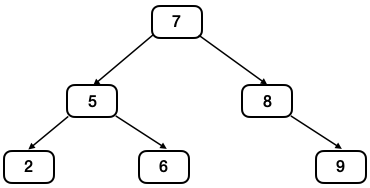
\includegraphics[scale=0.5]{assets/img/bst.png}
    \end{figure}
\end{frame}

\section{Conclusioni}
\begin{frame}{Considerazioni finali}
\begin{itemize}
    \item L'impiego di un SMT solver rende il processo di verifica opaco
    \item "Effetto farfalla" durante la prova
    \item Un SMT solver non è un oracolo, i limiti al calcolo rimangono
    \item Alcuni limiti del calcolo possono essere superati da accortezze nel linguaggio (quantificatori)
    \item Il linugaggio può essere utilizzato anche come \textit{proof assistant} attraverso lemmi e \textit{calc}
\end{itemize}
\end{frame}

\begin{frame}{Bibliografia}
    \Fontvi
    \bibliographystyle{plain}
    \bibliography{Bibliography}
\end{frame}


\end{document}
